\subsection{FactorGraph}

The FactorGraph class represents a single factor graph and contains a collection of all factors associated with that factor graph and all variables that are connected by factors to the graph.

\subsubsection{Constructor}

\begin{lstlisting}
FactorGraph([boundaryVariables])
\end{lstlisting}

For a basic factor graph, the constructor is simply the command FactorGraph with no arguments.

For a nested factor graph (one that may be used as a sub-graph within another graph), the constructor must include a list of the boundary variables of the graph.  When used as a sub-graph, the boundary variables are dummy variables with the same specification as the variables in the outer graph that will ultimately connect to the sub-graph.  A graph defined with boundary variables may alternatively be used as a top-level graph, in which case the boundary variables are used directly.

\subsubsection{Properties}

\para{Solver}
\label{sec:FactorGraph.Solver}

Read-write.  Indicates the choice of solver to be used for performing inference on the graph.  The default solver is SumProduct.

When setting the solver, the solver is given by a string representing the name of the solver.  The solver name is case insensitive.

\begin{lstlisting}
fg.Solver = 'SolverName';
\end{lstlisting}

The current set of valid solver names are:

\begin{itemize}
\item SumProduct
\item MinSum
\item Gaussian
\item ParticleBP
\item Gibbs
\end{itemize}

A description of each of these solvers is given in section~\ref{sec:SolversAPI}.

Note that the solver can be modified at any time.  After running the solver on a graph, the solver may be modified and the new solver run using the same graph\footnote{In this case, care must be taken to set any solver-specific parameters to the new values after changing the solver.}.  One exception is that if solver-specific built-in factors (also referred to as ``custom factors'') are used in a graph, it is not possible to switch solvers (a list of solver-specific built-in factors is given at the end of section~\ref{sec:builtInFactors}).


\para{Scheduler}
\label{sec:FactorGraph.Scheduler}

Read-write.  Indicates the scheduler to be used for performing inference on the graph (unless a custom schedule is specified instead).

When setting the scheduler, the scheduler is given by a string representing the name of the scheduler.  The scheduler name is case \emph{sensitive}.

\begin{lstlisting}
fg.Scheduler = 'SchedulerName';
\end{lstlisting}

For all of the BP solvers (SumProduct, MinSum, Gaussian, ParticleBP), the following schedulers are available:

\begin{longtable}{l p{4in}}
\textbf{Name} & \textbf{Description} \\ \hline \hline
%
\textsf{DefaultScheduler} & Same as the TreeOrFloodingScheduler, which is the default if no scheduler or custom schedule is specified. \\ \hline
%
\textsf{TreeOrFloodingScheduler} & The solver will use either a Tree Schedule or a Flooding Schedule depending on whether the factor-graph contains cycles.  In a nested graph, this choice is applied independently in each subgraph.  If the factor-graph is a tree, the scheduler will automatically detect this and use a Tree Schedule.  In this schedule, each node is updated in an order that will result in the correct beliefs being computed after just one iteration.  If the entire graph is a tree, NumIterations should be set to 1, which is its default value.  If the factor-graph is loopy, the solver will instead use a Flooding Schedule (as described below). \\ \hline
%
\textsf{TreeOrSequentialScheduler} & The solver will use either a Tree Schedule (as described above) or a Sequential Schedule (as described below) depending on whether the factor-graph contains cycles.  In a nested graph, this choice is applied independently in each subgraph.  \\ \hline
%
\textsf{FloodingScheduler} & The solver will apply a Flooding Schedule.  For each iteration, all variable nodes are updated, followed by all factor nodes.  Because the graph is bipartite (factor nodes only connect to variable nodes, and vice versa), the order of update within each node type does not affect the result. \\ \hline
%
\textsf{SequentialScheduler} & The solver will apply a Sequential Schedule.  For each factor node in the graph, first, for each variable connected to that factor, the edge connecting the variable to the factor is updated; then the factor node is updated.  The specific order of factors chosen is arbitrary, and depends on the order that factors were added to the graph. \\ \hline
%
\textsf{RandomWithoutReplacementScheduler} & The solver will apply a Sequential Schedule with the order of factors chosen randomly without replacement.  On each subsequent iteration, a new random order is chosen.  Since the factor order is chosen randomly with replacement, on each iteration, each factor will be updated exactly once. \\ \hline
%
\textsf{RandomWithReplacementScheduler} & The solver will apply a Sequential Schedule with the order of factors chosen randomly with replacement.  On each subsequent iteration, a new random order is chosen.  The number of factors updated per iteration is equal to the total number of factors in the graph. However, since the factors are chosen randomly with replacement, not all factors are necessarily updated in a single iteration, and some may be updated more than once. \\ \hline
%
\end{longtable}


In a nested graph, for most of the schedulers listed above (except for the random schedulers), the schedule is applied hierarchically.  In particular, a subgraph is treated as a factor in the nesting level that it appears.  When that subgraph is updated, the schedule for the corresponding subgraph is run in its entirety, updating all factors and variables contained within according to its specified schedule.

It is possible for subgraphs to be designated to use a schedule different from that of its parent graph.  This can be done by specifying either a scheduler or a custom schedule for the subgraph prior to adding it to the parent graph.  For example:
%
\begin{lstlisting}
SubGraph.Scheduler = 'SequentialScheduler';
ParentGraph.addFactor(SubGraph, boundaryVariables);
ParentGraph.Scheduler = 'FloodingScheduler';
\end{lstlisting}

For the TreeOrFloodingScheduler and the TreeOrSequentialScheduler, the choice of schedule is done independently in the outer graph and in each subgraph.  In case that a subgraph is a tree, the tree scheduler will be applied when updating that subgraph even if the parent graph is loopy.  This structure can improve the performance of belief propagation by ensuring that the effect of variables at the boundary of the subgraph fully propagates to all other variables in the subgraph on each iteration.

For the RandomWithoutReplacementScheduler and RandomWithReplacementScheduler, if these are applied to a graph or subgraph, the hierarchy of any lower nesting layers is ignored.  That is, the subgraphs below are essentially flattened prior to schedule creation, and any schedulers or custom schedules specified in lower layers of the hierarchy are ignored.


Because of the differences in operation between the Gibbs solver and the BP based solvers, the Gibbs solver supports a distinct set of schedulers.  For the Gibbs solver, the following schedulers are available:

\begin{tabular}{l p{4in}}
\textbf{Name} & \textbf{Description} \\ \hline \hline
%
\textsf{GibbsDefaultScheduler} & Same as the GibbsSequentialScanScheduler, which is the default when using the Gibbs solver. \\ \hline
%
\textsf{GibbsSequentialScanScheduler} & The solver will apply a Sequential Scan Schedule.  For each scan, each variable is resampled in a fixed order.  The specific order of variables chosen is arbitrary, and depends on the order that variables were added to the graph. \\ \hline
%
\textsf{GibbsRandomScanScheduler} & The solver will apply a Random Scan Schedule.  Each successive variable to be resampled is chosen randomly with replacement.  The number of variables resampled per scan is equal to the total number of variables in the graph, but not all variables are necessarily resampled in a given scan, and some may be resampled more than once. \\ \hline
%
\end{tabular}

Because of the nature of the Gibbs solver, the nested structure of a graph is ignored in creating the schedule.  That is, the graph hierarchy is essentially flattened prior to schedule creation, and only the scheduler specified on the outermost graph is applied.



\para{Schedule}
\label{sec:FactorGraph.Schedule}

Read-write.  Specifies a custom schedule to be used for performing inference.


\para{NumIterations}

Read-write.  The NumIterations property sets the number of iterations BP will to run when using the solve method.  This only applies to solvers that use BP, which are the SumProduct, MinSum, Gaussian, and ParticleBP solvers.

The default value is 1.  For a factor graph with a tree-structure, when using the default scheduler, one iteration is appropriate.  Otherwise, it would normally be appropriate to set the number of iterations to a larger value.

\para{NumSteps}

\para{Name}

Read-write.  When read, retrieves the current name of the factor graph.  When set, modifies the name of the factor graph to the corresponding value.  The value set must be a string.

\begin{lstlisting}
fg.Name = 'string';
\end{lstlisting}


%\para{QualifiedName}
%
%\para{ExplicitName}
%
%\para{Label}
%
%\para{QualifiedLabel}
%
%\para{UUID}
%
%\para{Nodes}
%
%\para{NodesFlat}
%
%\para{NodesTop}
%
%\para{Variables}
%
%\para{VariablesFlat}
%
%\para{VariablesTop}
%
%\para{Factors}
%
%\para{FactorsFlat}
%
%\para{FactorsTop}
%
%\para{NonGraphFactors}
%
%\para{NonGraphFactorsFlat}
%
%\para{NonGraphFactorsTop}
%
%\para{NestedGraphs}
%
%\para{FactorGraphStreams}
%
%\para{AdjacencyMatrix}

\para{Score}

\para{BetheFreeEnergy}

\para{BetheEntropy}

\para{InternalEnergy}


\subsubsection{Methods}

\para{initialize}

\begin{lstlisting}
MyGraph.initialize();
\end{lstlisting}

The initialize method resets the state of the factor graph and its associated solver.  When performing inference incrementally, for example using the iterate method, the initialize method must be called before the first iterate call.  When using the solve method to perform inference, there is no need to call initialize first.  The initialize method takes not arguments.

\para{solve}

\begin{lstlisting}
MyGraph.solve();
\end{lstlisting}

The solve method runs the solver on the factor graph for the specified duration.  Calling solve initializes the graph prior to solving.


\para{addFactor}

The addFactor (and related) methods are used to add a factor to a factor-graph, connecting that factor to a specified set of variables.  There are several ways of specifying the particular factor:

\begin{itemize}
\item A MATLAB function handle.
\item A sub-graph.
\item A factor-table.
\item A built-in factor.
\item A built-in overloaded MATLAB operator.
\item A custom Java FactorFunction object.
\end{itemize}

Each of these methods is summarized in the subsequent sections.

\subpara{MATLAB Function Handle}

A factor may be specified by defining a MATLAB function, and passing a handle to that function.  The function must accept values that correspond to the state of the connected variables (in the same order as specified in the addFactor call), and return a non-negative weight corresponding to the unnormalized value of the factor.

In this case, the �addFactor� method takes the following arguments:

\begin{itemize}
\item A function handle. 
\item A variable length list of Variables or matrices.
\end{itemize}

For example,

\begin{lstlisting}
MyGraph.addFactor(@XorDeltaTutorial,x,y,z);	
\end{lstlisting}

The ``@'' symbol indicates a function handle, where the function ``XorDeltaTutorial'' is assumed to exist somewhere in the current MATLAB path.

Using a MATLAB function to specify a factor is valid in Dimple only when all of the connected variables are discrete (either Discrete or Bit).  Real values are allowed in other parts of a graph, as long as they are not directly connected to this factor.

Some of the variables in the call may be replaced by constants.  In this case, no variable is created, but instead the specified constant value is used for the value of that input to the factor function.  The following shows an example of mixing variables and constants as arguments to the addFactor method.

\begin{lstlisting}
b = Bit(2,1);
MyGraph.addFactor(@XorDeltaTutorial,b(1),1, b(2));	
\end{lstlisting}

The constants can be any n-dimensional real or complex matrix.  

Adding a Factor in this way involves creating an array known as a factor table, which contains all assignments of the variables resulting in a positive value of the function, along with a value vector, containing all the corresponding values of the function. This table is then passed to the solver. Creating that table takes time (and typically space) proportional to the product of the size of the domains of all variables connected to that factor, thus requiring an exponential time in the degree of the factor.  The addFactor method attempts to save memory and time by re-using existing factors when addFactor is called with the same factor function.  The caching mechanism uses the name of the function (using MATLAB�s func2str) as well as the domain values for all of the arguments to addFactor when deciding if a FactorTable can be re-used.  If this behavior is undesirable, the addFactorNoCache method can be used instead of addFactor (see below).

\subpara{Nested Graphs}

In a nested graph, a sub-graph can be added to its parent graph using the addFactor method.  In this case, the first argument of the addFactor call is the sub-graph.  For example:

\begin{lstlisting}
MyGraph.addFactor(mySubGraph, a, b, c);
\end{lstlisting}

The number and order of the variables must correspond to the number and order of the connector variables declared when the sub-graph was created.

\subpara{Specifying FactorTables}

For all discrete factors, Dimple can build FactorTables under the hood. A Factor Table consists of a two dimensional array of integers and a single dimensional array of doubles. Each row of the two dimensional table represents a combination of variables for which the Factor Function returns a non-zero value. Each column represents a variable connected to the factor. The values of the table specify an index into the discrete domain of a variable. Each row of the two dimensional table corresponds to one entry of the array of doubles and that entry contains the return value of the Factor Function.

In some situations, a user might be able to build a FactorTable much more efficiently than Dimple can. Dimple tries all combinations of variable values exhaustively and discards combinations for which the Factor Function returns zeros. If the user can avoid this exhaustive search, they can build the FactorTable more quickly.

Once the user has created the table, they can add a Factor using this table in one of two ways. The first is to provide the indices and values directly to the addFactor call:

\begin{lstlisting}
   %First let's just add the factor as indices and values
   fg = FactorGraph();
   b = Bit(2,1);
   ind = [0 0; 1 1];
   val = [1 1];
   fg.addFactor(ind,val,b);
   b(1).Input = .8;
   fg.solve();
   assertEqual(b(2).Belief,.8);
\end{lstlisting}
   
Notice that the indices and values chosen here will be equivalent to creating an equals factor between the two variables. In the following example we see that it's possible to first create a Table and then add a factor using that table. This has the advantage of using less overall memory if this same table will be used in multiple factors.

\begin{lstlisting}
   %Now let's add the Factor using createTable to test we can share tables
   fg = FactorGraph();
   b = Bit(2,1);   
   t = FactorTable(ind,val,b.Domain,b.Domain);	
   fg.addFactor(t,b);
   b(1).Input = .8;
   fg.solve();
   assertEqual(b(2).Belief,.8);
\end{lstlisting}

Users can also create a FactorTable given a single n-dimensional matrix such that: $ val(x_1,...,x_n) = F(d_1(x_11),...,d_n(x_n)) $

Where val is the N dimensional matrix, F is the desired Factor Function, and di is a function mapping 1 based indices to domain elements of domain i.  This will result in an uncompressed table, so it doesn�t offer a speed improvement, but provides a convenient way to create Factors in some cases.

\begin{lstlisting}
   fg = FactorGraph();
   b = Bit(2,1);
   val = [1 0; 0 1];
   t = FactorTable(val,b.Domain,b.Domain);
   fg.addFactor(t,b);
   b(1).Input = .8;
   fg.solve();
   assertEqual(b(2).Belief,.8);
\end{lstlisting}

or equivalently:

\begin{lstlisting}
   fg = FactorGraph();
   b = Bit(2,1);
   val = [1 0; 0 1];
   fg.addFactor(val,b);
   b(1).Input = .8;
   fg.solve();
   assertEqual(b(2).Belief,.8);
\end{lstlisting}

In yet another way to specify FactorTables, users can create an empty Factor Table and use the �set� function to set values at specified domain combinations.

\begin{lstlisting}
   fg = FactorGraph();
   b = Discrete({'on','off'},2,1);
   t = FactorTable(b.Domain,b.Domain);
   t.set('on','on',1);
   t.set('off','off',1);
   fg.addFactor(t,b);
   b(1).Input = [.8 .2];
   fg.solve();
   assertEqual(b(2).Belief(1),.8);
\end{lstlisting}

Users can retrieve values using the FactorTable �get� function.

\begin{lstlisting}
>> t.get('on','on')

ans =

     1
\end{lstlisting}


\subpara{Built-in Factors}
\label{sec:builtInFactors}

Dimple supports a set of built-in factors that can be specified when adding a factor to a graph.  When calling the addFactor method, in many cases, the user may specify these functions by name (which is case sensitive).  In some cases, there are optional arguments for these built-in factor, in which case an alternative syntax must be used (see below).

As an example,

\begin{lstlisting}
Mean = Real();
InverseVariance = Real();
Values = Real(1,100);
MyGraph.addFactor('Normal', Mean, InverseVariance, Values);
\end{lstlisting}

The following table lists the current set of built-in Dimple factors.  For each, the name is given, followed by the set of variables that would be connected to the factor, followed by any constructor arguments.  Optional variables and constructor arguments are in brackets.  And an arbitrary length list or vector of variables is followed by ellipses.  The allowed set of variable data-types for each variable is given in parentheses (B = Bit, D = Discrete, or R = Real).  If no list is shown, then any data-type may be used.

\begin{longtable} {l p{2.2cm} p{2cm} p{7cm}}
Name & Variables & Constructor & Description \\
\hline
\endhead
%
Abs & out(D,R) \newline in(D,R) & [smoothing] & Deterministic absolute value function, where out = abs(in).  An optional smoothing value may be specified as a constructor argument\footnote{\label{ftn:smoothing}If smoothing is enabled, the factor function becomes $e^{-(\textrm{out} - F(\textrm{in}))^2/\textrm{smoothing}}$ (making it non-deterministic) instead of $\delta(\textrm{out} - F(\textrm{in}))$, where $F$ is the deterministic function associated with this factor.  This is useful for solvers that do not work well with deterministic real-valued factors, such as particle BP, particularly when tempering is used.}.\\
%
ACos & out(D,R) \newline in(D,R) & [smoothing] & Deterministic arc-cosine function, where out = acos(in). An optional smoothing value may be specified as a constructor argument$^{\ref{ftn:smoothing}}$. \\
%
AdditiveNoise & out(R) \newline in(B,D,R) & $\sigma$ & Add Gaussian noise with a known standard deviation, $\sigma$, specified in constructor. \\
%
And & out(B) \newline in...(B) & - & Deterministic logical AND function, where out = AND(in...). \\
%
ASin & out(D,R) \newline in(D,R) & [smoothing] & Deterministic arc-sine function, where out = asin(in). An optional smoothing value may be specified as a constructor argument$^{\ref{ftn:smoothing}}$. \\
%
ATan & out(D,R) \newline in(D,R) & [smoothing] & Deterministic arc-tangent function, where out = atan(in). An optional smoothing value may be specified as a constructor argument$^{\ref{ftn:smoothing}}$. \\
%
Beta & [$\alpha$](R) \newline [$\beta$](R) \newline value...(R) & [$\alpha$] \newline [$\beta$] & Beta distribution. There can be any number of value variables, all associated with the same parameter values.  Parameters $\alpha$ and $\beta$ can be variables, or if both are constant they can be specified in the constructor. \\
%
Categorical & $\alpha$...(R)  \newline x...(D) & N & Categorical distribution, $p(x | \alpha)$, where $\alpha$ is a vector of parameter variables and x is a vector of discrete variables.  The number of elements in $\alpha$ and the domain size of x must equal the value of the constructor argument, N.  There can be any number of x variables, all associated with the same parameter values.  \newline
The $\alpha$ parameters are represented as energy values, that is, $\alpha = -\log(\rho)$, where $\rho$ are unnormalized probabilities. The conjugate prior for this representation is such that each entry of $\alpha$ is independently distributed according to a negative exp-Gamma distribution, all with a common $\beta$ parameter (it is not necessary to use the conjugate prior, but in some cases there may be a benefit).  \newline
In the current implementation, the domain of the x variable must be zero-based contiguous integers, $0...N-1$ (this limitation may be lifted in a future version). \\
%
ConstantPower & out(D,R) \newline base(D,R) & power \newline [smoothing] & Deterministic power function, with a constant power. The power value is specified in the constructor. An optional smoothing value may be specified as a constructor argument$^{\ref{ftn:smoothing}}$. \\
%
ConstantProduct & out(D,R) \newline in(D,R) & constant \newline [smoothing] &  Deterministic product function, multiplying the input times a constant value.  The constant value is specified in the constructor. An optional smoothing value may be specified as a constructor argument$^{\ref{ftn:smoothing}}$. \\
%
Cos & out(D,R) \newline in(D,R) & [smoothing] & Deterministic cosine function, where out = cos(in). An optional smoothing value may be specified as a constructor argument$^{\ref{ftn:smoothing}}$. \\
%
Cosh & out(D,R) \newline in(D,R) & [smoothing] & Deterministic hyperbolic-cosine function, where out = cosh(in). An optional smoothing value may be specified as a constructor argument$^{\ref{ftn:smoothing}}$. \\
%
DiscreteTransition & x(D) \newline y(D) \newline A(R) & $N_{x}, N_{y} | \newline N$ & 
Parameterized discrete transition factor, $p(y | x, A)$, where x and y are discrete variables, and $A$ is a matrix of transition probabilities. The transition matrix is organized such that columns correspond to the output distribution for each input state. That is, the transition matrix multiplies on the left. The number of columns in A and the domain size of x must equal the value of the constructor argument, $N_{x}$ and the number of rows in A and the domain size of y must equal the value of the constructor argument $N_{y}$.  If $N_{x}$ and $N_{y}$ are equal, a single constructor argument, $N$, may be used.  \newline
The elements of the matrix A are represented as energy values, that is, $A_{i,j} = -\log(\rho_{i,j})$, where $\rho$ is an unnormalized transition probability matrix.  The conjugate prior for this representation is such that each entry of A is independently distributed according to a negative exp-Gamma distribution, all with a common $\beta$ parameter (it is not necessary to use the conjugate prior, but in some cases there may be a benefit).  \newline
In the current implementation, the domain of the x variable must be zero-based contiguous integers, $0...N-1$ (this limitation may be lifted in a future version). \\
%
Divide & quotient(D,R) \newline dividend(D,R) \newline divisor(D,R) & [smoothing] & Deterministic divide function, where $\mathrm{quotient} = \frac{\mathrm{dividend}}{\mathrm{divisor}}$. An optional smoothing value may be specified as a constructor argument$^{\ref{ftn:smoothing}}$. \\
%
Equality & value...(B,D,R) & [smoothing] & Deterministic equality constraint.  An optional smoothing value may be specified as a constructor argument$^{\ref{ftn:smoothing}}$. \\
%
Equals & out(B) \newline in...(B,D,R) & - & Deterministic equals function, where out~=~(in(1)~==~in(2)~== ... ). \\
%
Exp & out(D,R) \newline in(D,R) & [smoothing] & Deterministic exponentiation function, where out = exp(in). An optional smoothing value may be specified as a constructor argument$^{\ref{ftn:smoothing}}$. \\
%
Gamma & [$\alpha$](R) \newline [$\beta$](R) \newline value...(R) & [$\alpha$] \newline [$\beta$] & Gamma distribution. There can be any number of value variables, all associated with the same parameter values.  Parameters $\alpha$ and $\beta$ can be variables, or if both are constant they can be specified in the constructor. \\
%
GreaterThan & out(B) \newline in1(B,D,R) \newline in2(B,D,R) & - & Deterministic greater-than function, where out = in1 $>$ in2.  \\
%
InverseGamma & [$\alpha$](R) \newline [$\beta$](R) \newline value...(R) & [$\alpha$] \newline [$\beta$] & Inverse Gamma distribution. There can be any number of value variables, all associated with the same parameter values.  Parameters $\alpha$ and $\beta$ can be variables, or if both are constant they can be specified in the constructor. \\
%
LessThan & out(B) \newline in1(B,D,R) \newline in2(B,D,R) & - & Deterministic greater-than function, where out = in1 $<$ in2.  \\
%
LinearEquation & out(D,R) \newline in(B,D,R) & constants \newline [smoothing] & Deterministic linear equation, multiplying an input vector by a constant vector. The constant vector is specified in the constructor.  The number of \emph{in} variables must equal the length of the constant vector. An optional smoothing value may be specified as a constructor argument\textsuperscript{\ref{ftn:smoothing}}. \\
%
Log & out(D,R) \newline in(D,R) & [smoothing] & Deterministic natural log function, where out = log(in). An optional smoothing value may be specified as a constructor argument$^{\ref{ftn:smoothing}}$. \\
%
LogNormal & [$\mu$](R) \newline [$\tau$](R) \newline value...(R) & [$\mu$] \newline [$\tau$] & Log-normal distribution. There can be any number of value variables, all associated with the same parameter values.  Parameters $\mu$ (mean) and $\tau = \frac{1}{\sigma^{2}}$ (precision) can be variables, or if both are constant then fixed parameters can be specified in the constructor. \\
%
MatrixVectorProduct & y(D,R) \newline M(D,R) \newline x(D,R) & $N_{x}$ \newline $N_{y}$ \newline [smoothing] & Deterministic matrix-vector product function, $y = Mx$, where $x$ and $y$ are vectors and $M$ is a matrix. Constructor arguments, $N_{x}$ and $N_{y}$, specify the input and output vector lengths, respectively. The matrix dimension is $N_{y} \times N_{x}$. An optional smoothing value may be specified as a constructor argument$^{\ref{ftn:smoothing}}$. \\
%
MixedNormal & value(R) \newline control(B) & $\mu_{0} \newline \tau_{0} \newline \mu_{1} \newline \tau_{1}$ & Simple mixture of two fixed-parameter Normal distributions. The choice of distribution parameters (0 vs. 1) is a function of the control bit. \\
%
Negate & out(D,R) \newline in(D,R) & [smoothing] & Deterministic negation function, where out = -in. An optional smoothing value may be specified as a constructor argument$^{\ref{ftn:smoothing}}$. \\
%
NegativeExpGamma & [$\alpha$](R) \newline [$\beta$](R) \newline value...(R) & [$\alpha$] \newline [$\beta$] & Negative exp-Gamma distribution, which is a distribution over a variable whose negative exponential is Gamma distributed. That is, this is the negative log of a Gamma distributed variable. There can be any number of value variables, all associated with the same parameter values.  Parameters $\alpha$ and $\beta$ can be variables, or if both are constant they can be specified in the constructor, and correspond to the parameters of the underlying Gamma distribution. \\
%
Normal & [$\mu$](R) \newline [$\tau$](R) \newline value...(R) & [$\mu$] \newline [$\tau$] & Normal distribution. There can be any number of value variables, all associated with the same parameter values.  Parameters $\mu$ (mean) and $\tau = \frac{1}{\sigma^{2}}$ (precision) can be variables, or if both are constant then fixed parameters can be specified in the constructor. \\
%
Not & out(B) \newline in(B) & - & Deterministic logical NOT of function, where out = ~in. \\
%
NotEquals & out(B) \newline in...(B,D,R) & - & Deterministic not-equals function, where out~=~$\sim$(in(1)~==~in(2)~== ... ). \\
%
Or & out(B) \newline in...(B) & - & Deterministic logical OR function, where out = OR(in...). \\
%
Power & out(D,R) \newline base(D,R) \newline power(D,R) & [smoothing] & Deterministic power function, where out~=~base~$^{\mathrm{power}}$. An optional smoothing value may be specified as a constructor argument$^{\ref{ftn:smoothing}}$. \\
%
Product & out(D,R) \newline in...(B,D,R) & [smoothing] & Deterministic product function, where $\mathrm{out} = \prod \mathrm{in}$. An optional smoothing value may be specified as a constructor argument$^{\ref{ftn:smoothing}}$. \\
%
Rayleigh & [$\sigma$](R) \newline value...(R) & [$\sigma$] & Rayleigh distribution. There can be any number of value variables, all associated with the same parameter value.  Parameter $\sigma$ can be a variable, or if constant, can be specified in the constructor. \\
%
Sin & out(D,R) \newline in(D,R) & [smoothing] & Deterministic sine function, where out = sin(in). An optional smoothing value may be specified as a constructor argument$^{\ref{ftn:smoothing}}$. \\
%
Sinh & out(D,R) \newline in(D,R) & [smoothing] & Deterministic hyperbolic-sine function, where out = sinh(in). An optional smoothing value may be specified as a constructor argument$^{\ref{ftn:smoothing}}$. \\
%
Sqrt & out(D,R) \newline in(D,R) & [smoothing] & Deterministic square root function, where out = sqrt(in). An optional smoothing value may be specified as a constructor argument$^{\ref{ftn:smoothing}}$. \\
%
Square & out(D,R) \newline in(D,R) & [smoothing] & Deterministic square function, where out = in$^{2}$. An optional smoothing value may be specified as a constructor argument$^{\ref{ftn:smoothing}}$. \\
%
Subtract & out(D,R) \newline posIn(B,D,R) \newline negIn...(B,D,R) & [smoothing] & Deterministic summation function, where $\mathrm{out} = \mathrm{posIn} - \sum \mathrm{negIn}$. An optional smoothing value may be specified as a constructor argument$^{\ref{ftn:smoothing}}$. \\
%
Sum & out(D,R) \newline in...(B,D,R) & [smoothing] & Deterministic summation function, where $\mathrm{out} = \sum \mathrm{in}$. An optional smoothing value may be specified as a constructor argument$^{\ref{ftn:smoothing}}$. \\
%
Tan & out(D,R) \newline in(D,R) & [smoothing] & Deterministic tangent function, where out = tan(in). An optional smoothing value may be specified as a constructor argument$^{\ref{ftn:smoothing}}$. \\
%
Tanh & out(D,R) \newline in(D,R) & [smoothing] & Deterministic hyperbolic-tangent function, where out = tanh(in). An optional smoothing value may be specified as a constructor argument$^{\ref{ftn:smoothing}}$. \\
%
VonMises & [$\mu$](R) \newline [$\tau$](R) \newline value...(R) & [$\mu$] \newline [$\tau$] & Von Mises distribution. There can be any number of value variables, all associated with the same parameter values.  Parameters $\mu$ (mean) and $\tau = \frac{1}{\sigma^{2}}$ (precision) can be variables, or if both are constant then fixed parameters can be specified in the constructor.  The distribution is non-zero for value variables in the range $-\pi$ to $\pi$. \\
%
Xor & out(B) \newline in...(B) & - & Deterministic logical XOR function, where out = XOR(in...). \\
%
\end{longtable}

The above factors may be specified by name if no constructor arguments are needed.  If constructor arguments are needed, then there are two ways to specify the factor.  The preferred way is to create a FactorFunction object, which takes the name of the factor followed by the constructor arguments for that factor.  For example:

\begin{lstlisting}
MyGraph.addFactor(FactorFunction('Gamma', 1, 1), X);
\end{lstlisting}

The same FactorFunction can be used more than once, which avoids creating additional copies of the FactorFunction object.  For example:

\begin{lstlisting}
myFactorFunction = FactorFunction('Gamma', 1, 1);
MyGraph.addFactor(myFactorFunction, X1);
MyGraph.addFactor(myFactorFunction, X2);
\end{lstlisting}

A short-hand notation may alternatively be used, in which the name of the factor function and its constructor arguments are contained in a cell array.  For example:

\begin{lstlisting}
MyGraph.addFactor({'Gamma', 1, 1}, X);
\end{lstlisting}


In addition to the built-in factors listed above, there are a set of solver-specific built-in factors, also referred to as ``custom factors.''  These factors may also be specified by name in the addFactor call (using either a quoted string or as a function handle).  These are summarized in the following table:

\begin{longtable} {l p{3cm} p{7cm}}
Name & Solver & Description \\
\hline
\endhead
%
FiniteFieldFactor & SumProduct\footnote{\label{ftn:fff} These may also be used for discrete variables with the Gaussian or particle BP solvers, which use the sum-product solver for discrete-only portions of the graph.}  & See section~\ref{sec:finiteFields} \\ 
FiniteFieldProjection & SumProduct$^{\ref{ftn:fff}}$ & See section~\ref{sec:finiteFields} \\ 
FiniteFieldAdd & SumProduct$^{\ref{ftn:fff}}$ & See section~\ref{sec:finiteFields} \\ 
FiniteFieldConstMult & SumProduct$^{\ref{ftn:fff}}$ & See section~\ref{sec:finiteFields} \\ 
FiniteFieldMult & SumProduct$^{\ref{ftn:fff}}$ & See section~\ref{sec:finiteFields} \\ 
CustomXor & MinSum & Same as the Xor factor described above, but with a significantly faster implementation. \\ 
\end{longtable}


Dimple also includes some built-in helper functions to create structured graphs, combining smaller factors to form an efficient implementation of a larger subgraph.  Specifically, the following functions are provided.

\begin{itemize}
\item getNBitXorDef(n), where n is a positive integer. Returns a nestable graph and an array of n-Bit connector variables. Efficient tree implementation of the XORDelta function.
\item getVXOR(n), where n is a positive integer. Returns a nestable graph and an array of n-Bits connector variables. Constrains exactly one bit to be 1, and all others to be 0.
\end{itemize}




\subpara{Adding Factors Implicitly Using MATLAB Operators or Functions}

Dimple supports a set of built-in factors that can be added implicitly using overloaded MATLAB operators or functions.  For example,

\begin{lstlisting}
fg = FactorGraph();
a = Discrete(1:4);
b = Discrete(1:10);
c = a + b;
\end{lstlisting}

The last line of this example will create a new variable, c, and a 'Sum' factor with variables c, a, and b.  The domain of c will be defined appropriately given the domains of the input variables.  In this example, the domain of c would automatically be set to the range [2:14].

These operations can be compounded in a single line of code, and variables of different data types as well as constants can be intermingled (as long as the type is supported by the specific operator).  In this case, intermediate anonymous variables will be created in the graph associated with intermediate results of the operation.  For example,

\begin{lstlisting}
z = (a + b) * c^d - sqrt(-e);
\end{lstlisting}

Like using the addFactor method, adding factors implicitly can include constants.  Specifically, for binary operators, one of the inputs may be a constant instead of a variable.  For example:

\begin{lstlisting}
x = a^2;
y = (a + b + 2) * 3;
\end{lstlisting}

Since adding a factor implicitly does not specifically refer to the factor graph, the graph to which these factors are added is also implicit.  In particular, these implicitly defined factors are added to the last factor graph that was created.  So, in the first example above, the factor would be added to fg, regardless of whether other factor graphs had previously been created.

The specific set of operators supported is given in section~\ref{sec:overloaded}.



\subpara{Specifying Java Factor Functions}
\label{sec:userJava}

There are some cases in which it is desirable to add a factor function that is defined in Java rather than MATLAB. Specific cases where this is desirable are:

\begin{itemize}
\item The user wants to use a sample-based solver. Dimple's sample based solvers must use Java Factor Functions in order to be able to call the Factor Function at runtime. This is partly because MATLAB does not officially support callbacks from Java to MATLAB and also because calls from Java to Java will be faster than those that cross a language boundary.
\item The user wants their code to run faster. MATLAB function calls are very slow as compared to java function calls.
The following sections provides the steps users must follow to add a Java Factor Function to their FactorGraph.
\end{itemize}


\subparaNoToc{Create a Class That Inherits from Java FactorFunction}
\label{sec:createJavaFactorFunction}

Users must extend the FactorFunction class. They have to provide two methods:

\begin{itemize}
\item A constructor that call's the parent constructor.
\item An eval function that returns a weight for each possible set of inputs.
\end{itemize}

\begin{lstlisting}
import com.analog.lyric.dimple.FactorFunctions.core.FactorFunction;

/*
 * This factor enforces equality between all variables and weights
 * elements of the domain proportional to their value
 */
public class BigEquals extends FactorFunction
{	
    public BigEquals() 
    {
	super("BigEquals");
    }
  
    @Override
    public double eval(Object... input) throws Exception 
    {
	if (input.length == 0)
	    return 0;
	else
	{
	    double first = (Double) input[0];
	    
	    for (int i = 1; i < input.length; i++)
	    {
	        if ((Double)input[i] != first)
		    return 0;
	    }
	    return first;   
	}
    }
}
\end{lstlisting}

\subparaNoToc{Compiling}

The new class must be compiled to class files. Users can optionally create a jar file. If using Eclipse, users can simply create a new project, create the new class, and the .class files will be created automatically.

\subparaNoToc{Adding Binary to MATLAB Path}

In MATLAB, the user must use the javaaddpath call to add the java files to the javaclasspath.

\begin{lstlisting}
javaaddpath('<path to my project>/MyFactorFunctions/bin');
\end{lstlisting}

or

\begin{lstlisting}
javaaddpath('<path to the jar>/myjar.jar');
\end{lstlisting}

\subpara{Using the Factor Function}

Users can now instantiate the FactorFunction and call addFactor with the instance.

\begin{lstlisting}
be = BigEquals();
fg = FactorGraph(); 
v = Variable({0,1,2},2,1);
fg.addFactor(be,v(1),v(2));
fg.solve();
v(1).Belief
\end{lstlisting}

Note that the BigEquals class was added to the default package, so we can just call:

\begin{lstlisting}
be = BigEquals();
\end{lstlisting}

The previous code results in the following answer from MATLAB:

\begin{lstlisting}
ans =

   0.0000    0.3333    0.6667
\end{lstlisting}

\subparaNoToc{Re-using the Factor Function}
We can re-use the BigEquals() FactorFunction multiple times within a single graph or across graphs. This will result in caching of FactorTables when the arguments to the addFactor function have identical domains.

\begin{lstlisting}
be = BigEquals();
fg = FactorGraph(); 
v = Variable({0,1,2},2,1);
fg.addFactor(be,v(1),v(2));
fg.solve();
v(1).Belief

fg2 = FactorGraph();
v2 = Variable({0,1,2},2,1);
fg2.addFactor(be,v2(1),v2(2));
fg2.solve();
v2(1).Belief
\end{lstlisting}


\subpara{Constants}

Users can pass constants to addFactor.  The following passes the constant 1 to the xorDelta factor function as the final argument.

\begin{lstlisting}
fg = FactorGraph();
b = Bit(10,3);
fg.addFactorVectorized(@xorDelta,{b 1},1);
\end{lstlisting}


\para{addFactorNoCache}
\label{sec:addFactorNoCache}

There are several cases where Dimple�s factor caching mechanism is undesirable.  As an example, if the user is calling addFactor with the same factor many times, but they know the arguments are unique, they can save time by skipping the code that searches for a match in the cache. 

\begin{lstlisting}
fg = FactorGraph(); 
func = @(x,y) 1;
b = Bit(2,1);
for i=1:1000
fg.addFactorNoCache(func,b,rand());
end
\end{lstlisting}

This is a somewhat contrived example but, in this case, replacing addFactorNoCache with addFactor will significantly slow down the code.




\para{addFactorVectorized}

To get reasonable speed out of MATLAB, one needs to vectorize their code.  If a user wishes to build a FactorGraph with large numbers of factors in a regular arrangement, they will want to avoid making many calls to addFactor.  The addFactorVectorized method can be used instead to create many factors at once.

\subpara{Vectorizing over All Variables}

In this first example, we create three variable matrices and generate 12 factors connecting a(i,j), b(i,j), and c(i,j) for all i and j.

\begin{lstlisting}
fg = FactorGraph();
a = Bit(3,4);
b = Bit(3,4);
c = Bit(3,4);
fg.addFactorVectorized(@xorDelta,a,b,c);
\end{lstlisting}

\subpara{Specify Vectorize Dimensions}

By default addFactorVectorized will add factors for every dimension.  However, if a user wants to only vectorize over a subset of dimensions, addFactorVectorize
allows them to provide a cell array containing a variable matrix as the first argument and a list of dimensions to vectorize over as the second argument.  The following code will vectorize over the first two dimensions to create 12 xor factors.  Each xor factor is connected to 5 bits.

\begin{lstlisting}
fg = FactorGraph();
b = Bit(3,4,5);
fg.addFactorVectorized(@xorDelta,{b,[1 2]});
\end{lstlisting}

\subpara{Connecting a single variable with addFactorVectorized}

The addFactorVectorized method will ensure that dimensions being vectorized match for all inputs.  However, the call allows single variables to be connected to many as follows:

\begin{lstlisting}
fg = FactorGraph();
a = Bit(10,1);
b = Bit();
fg.addFactorVectorized(@xorDelta,a,b);
\end{lstlisting}

This will create a graph such that b is connected to every element of a via a total of 10 factors.

\subpara{repmat}

Similar things can be done with repmat.  Suppose you have a 10x1 vector of variables that you want connected to a 10x20 matrix of different variables.
The following code will create 200 factors.  Each element of a will be connected to 20 elements of b via 20 factors.

\begin{lstlisting}
fg = FactorGraph();
a = Bit(10,1);
b = Bit(10,20);
fg.addFactorVectorized(@xorDelta,repmat(a,1,10),b);
\end{lstlisting}

\para{Nested Graphs}

Nested Graphs are also supported

\begin{lstlisting}
a = Bit(3,1);
ng = FactorGraph(a);
ng.addFactor(@xorDelta,a);
fg = FactorGraph();
b = Bit(10,3);
fg.addFactorVectorized(ng,{b, 1});
\end{lstlisting}


\para{Adding Vectorized Factors Implicitly Using MATLAB Operators or Functions}

Adding built-in factors implicitly using overloaded MATLAB operators or functions can also be vectorized, with some limitations.  Specifically, if each of the input variables are vectors of the same dimension, then the result will be to create a vector of output variables of the same dimension, along with a vector of factors relating the inputs and outputs.

In some cases, to be consistent with MATLAB notation, there is a distinction made between the vectorized and non-vectorized operator.  Specifically, Dimple uses MATLAB's notation for point wise product and power operators to indicate a vectorized operation (currently using the matrix version of these operators on vector inputs is not supported).  For example, if variables a through e are vectors of variables of identical size, then the following would create a variable vector z, and a series of factors relating these variables.

\begin{lstlisting}
z = (a .* b) + c.^d - sqrt(-e);
\end{lstlisting}

For binary operators, one of the inputs may be a scalar variable or a scalar constant instead of a variable vector.  For a scalar variable, the result is that scalar variable connecting to each instance of the factors that are created.  For a constant, each instance of the factor uses the same constant for that input (vectors of distinct constants are not currently supported).  As an example:

\begin{lstlisting}
a = Real();
b = Discrete(domain, 1, 10);
z = a + b;					
\end{lstlisting}

The specific set of operators supported is given in section~\ref{sec:overloaded}.




\para{addDirectedFactor}

\para{addFactorNoCache}

\para{addRepeatedFactor}

\para{setSolver}
\para{Using a Name}

Dimple has been modified to allow users to register commonly used solvers so that they can be assigned using shorter names. Previously users had to do:

\begin{lstlisting}
setSolver(com.analog.lyric.dimple.solvers.sumproduct.Solver());
fg = FactorGraph();
\end{lstlisting}

or

\begin{lstlisting}
fg = FactorGraph();
fg.Solver = com.analog.lyric.dimple.solvers.sumproduct.Solver();
Users can now do:
setSolver('SumProduct'); 
fg = FactorGraph();
\end{lstlisting}

or

\begin{lstlisting}
fg = FactorGraph();
fg.Solver = 'SumProduct';
\end{lstlisting}

When setting the solver by name, the name is case insensitive.

For solvers that take constructor arguments, users can use the setSolver command:

\begin{lstlisting}
fg = FactorGraph();
fg.setSolver('Gibbs',param1,param2,param3,param4);
\end{lstlisting}

or

\begin{lstlisting}
setSolver('Gibbs',param1,param2,param3,param4);
\end{lstlisting}

For a full list of registered solvers, type:

\begin{lstlisting}
getSolverNames()
\end{lstlisting}

If users wish to register their own solvers they can call:

\begin{lstlisting}
registerSolver(solverName,solverConstructor);
\end{lstlisting}

And if they wish to unregister a solver they can call:

\begin{lstlisting}
unregisterSolver(solverName);
\end{lstlisting}




\para{advance}

\para{hasNext}

\para{solveOneStep}

\para{continueSolve}

\para{baumWelch}

\para{estimateParameters}

\para{join}

\para{split}

\para{removeFactor}

\para{plot}

%\para{getVariableByName}
%
%\para{getVariableByUUID}
%
%\para{getFactorByName}
%
%\para{getFactorByUUID}
%
%\para{getGraphByName}
%
%\para{getGraphByUUID}
%
%\para{isTree}
%
%\para{isTreeFlat}
%
%\para{isTreeTop}
%
%\para{isAncestorOf}
%
%\para{depthFirstSearch}
%
%\para{depthFirstSearchFlat}
%
%\para{depthFirstSearchTop}
%
%\para{getFactorGraphDiffsByName}
%
%\para{getAdjacencyMatrix}
%
%\para{getAdjacencyMatrixFlat}
%
%\para{getAdjacencyMatrixTop}
%
%\para{getAdjacencyString}
%
%\para{getNodeString}
%
%\para{getFullString}
%
%\para{disp}







\subsubsection{List of Overloaded MATLAB Operators and Functions}
\label{sec:overloaded}

The following table lists the set of overloaded MATLAB operators that can be used to implicitly create factors.  The table shows the operator, the corresponding factor, the valid variable data types of the inputs and outputs (B = Bit, D = Discrete, or R = Real), and wether or not vectorized inputs are supported.

\begin{longtable} {l p{3cm} p{1cm} p{1cm} p{1cm} l p{4cm}}
Operator & Factor & Out & In1 & In2 & Vectorized & Description \\
\hline
\endhead
%
$\&$ & And & B & B & B & \checkmark & Logical AND \\
$|$ & Or & B & B & B & \checkmark & Logical OR \\
xor() & Xor & B & B & B & \checkmark & Logical XOR \\
$\sim$ & Not & B & B & - & \checkmark & Logical NOT \\
$+$ & Sum & D,R\footnote{\label{ftn:outReal}If either input is Real, then the output is Real} & D,R & D,R & \checkmark & Plus \\
$-$ & Subtract & D,R\textsuperscript{\ref{ftn:outReal}} & D,R & D,R & \checkmark & Minus \\
$-$ & Negate & D,R\textsuperscript{\ref{ftn:outReal}} & D,R & - & \checkmark & Unary minus \\
$*$ & Product \newline MatrixVectorProduct & D,R\textsuperscript{\ref{ftn:outReal}} & D,R & D,R & \checkmark\footnote{One of the inputs may be a vector as long as the other is a scalar.} & Scalar multiply, or matrix-vector multiply\footnote{If one input is a vector and the other is a matrix of appropriate dimension, then the MatrixVectorProduct factor will be used.  Otherwise the Product factor will be used.} \\
$.*$ & Product & D,R\textsuperscript{\ref{ftn:outReal}} & D,R & D,R & \checkmark & Point-wise multiply \\
$/$ & Divide & D,R\textsuperscript{\ref{ftn:outReal}} & D,R & D,R & \checkmark\footnote{The dividend may be a vector as long as the divisor is a scalar.} & Scalar divide \\
$./$ & Divide & D,R\textsuperscript{\ref{ftn:outReal}} & D,R & D,R & \checkmark & Point-wise divide \\
$\wedge$ & Power & D,R\textsuperscript{\ref{ftn:outReal}} & D,R & D,R & \checkmark\footnote{The base may be a vector as long as the exponent is a scalar.} & Scalar power \\
$.\wedge$ & Power & D,R\textsuperscript{\ref{ftn:outReal}} & D,R & D,R & \checkmark & Point-wise power \\
$<$ & LessThan & B & D,R & D,R & \checkmark & Less than \\
$>$ & GreaterThan & B & D,R & D,R & \checkmark & Greater than \\
$<=$ & GreaterThan\footnote{Uses GreaterThan factor, reversing the order.} & B & D,R & D,R & \checkmark & Less than or equal to \\
$>=$ & LessThan\footnote{Uses LessThan factor, reversing the order.} & B & D,R & D,R & \checkmark & Greater than or equal to \\
Equals() & Equals & B & B,D,R & B,D,R\footnote{\label{ftn:equals}This function is not limited to two inputs, but can take an arbitrary number of inputs} & \checkmark & Equals\footnote{Equivalent to the $==$ operator, but the $==$ operator is not overloaded for this purpose so that it can instead be used to determine whether or not two variables reference the same Dimple variable.} \\
NotEquals() & NotEquals & B & B,D,R & B,D,R$^{\ref{ftn:equals}}$ & \checkmark & Not equals\footnote{Equivalent to the $\sim=$ operator, but the $\sim=$ operator is not overloaded for this purpose so that it can instead be used to determine whether or not two variables reference the same Dimple variable.} \\
mod() & - & D  & D & D & \checkmark & Modulo function\footnote{Currently, the mod() operator supports discrete variables only, and it uses the MATLAB definition of mod on negative numbers.  This may be subject to change in future versions.} \\
abs() & Abs & D,R\textsuperscript{\ref{ftn:outReal}} & D,R & - & \checkmark & Absolute value \\
sqrt() & Sqrt & R & R & - & \checkmark & Square root \\
log() & Log & R & R & - & \checkmark & Natural log \\
exp() & Exp & R & R & - & \checkmark & Exponential function \\
sin() & Sin & R & R & - & \checkmark & Sine \\
cos() & Cos & R & R & - & \checkmark & Cosine \\
tan() & Tan & R & R & - & \checkmark & Tangent \\
asin() & ASin & R & R & - & \checkmark & Arc-sine \\
acos() & ACos & R & R & - & \checkmark & Arc-cosine \\
atan() & ATan & R & R & - & \checkmark & Arc-tangent \\
sinh() & Sinh & R & R & - & \checkmark & Hyperbolic sine \\
cosh() & Cosh & R & R & - & \checkmark & Hyperbolic cosine \\
tanh() & Tanh & R & R & - & \checkmark & Hyperbolic tangent \\
\end{longtable}


Dimple also includes some helper functions to create other built-in factors using a similar syntax to the overloaded MATLAB functions listed above.  As for other overloaded functions, above, Dimple automatically creates the factors as well as the output variable(s).  The built-in factors that support this syntax are:

\begin{itemize}
\item Beta
\item Gamma
\item InverseGamma
\item NegativeExpGamma
\item Normal
\item LogNormal
\item VonMises
\item Rayleigh
\item Categorical
\end{itemize}

For each, the arguments are the parameters of the distribution.  For example:

\begin{lstlisting}
W = Gamma(alpha, beta);
X = Normal(mean, precision);
Y = Categorical(alphaVector);
Z = Rayleigh(sigma);
\end{lstlisting}


The parameters can be variables, constants, or some of each.

By default, calling one of these functions creates a single output variable, and the factor is added to the most-recently created graph. �But, optional arguments allow you to specify the dimensions of the array of output variables, or to specify the factor graph. �These arguments can be in either order after the parameters. �For example:

\begin{lstlisting}
W = Gamma(alpha, beta, altGraph);
X = Normal(mean, precision, [100, 1]);
Y = Categorical(alphaVector, [10, 10, 2], aGraph);
Z = Rayleigh(sigma, myGraph, size(somethingElse));
\end{lstlisting}



\subsubsection{Setting the Solver}



\subsubsection{Setting the Scheduler}

The scheduler determines the schedule to apply when solving the graph, which is the order of updates of variables and factors.  The user may choose among one of several pre-defined schedulers using the Scheduler method.  Each scheduler examines the structure of the graph and applies a rule to determine the schedule that will be used.  Alternatively, the user may supply a custom schedule using the Schedule method (see section~\ref{sec:customSchedules}).

If no scheduler or custom schedule is specified, a default scheduler will be used.  The default scheduler depends on the selected solver.

A scheduler is specified as follows:
\begin{lstlisting}
MyGraph.Scheduler = 'ExampleScheduler';	
\end{lstlisting}

When setting the scheduler for a graph, the name of the scheduler is case sensitive.

For all solvers except for the Gibbs solver (SumProduct, MinSum, Gaussian, ParticleBP), the following schedulers are available:

\begin{longtable}{l p{4in}}
\textbf{Name} & \textbf{Description} \\ \hline \hline
%
\textsf{DefaultScheduler} & Same as the TreeOrFloodingScheduler, which is the default if no scheduler or custom schedule is specified. \\ \hline
%
\textsf{TreeOrFloodingScheduler} & The solver will use either a Tree Schedule or a Flooding Schedule depending on whether the factor-graph contains cycles.  In a nested graph, this choice is applied independently in each subgraph.  If the factor-graph is a tree, the scheduler will automatically detect this and use a Tree Schedule.  In this schedule, each node is updated in an order that will result in the correct beliefs being computed after just one iteration.  If the entire graph is a tree, NumIterations should be set to 1, which is its default value.  If the factor-graph is loopy, the solver will instead use a Flooding Schedule (as described below). \\ \hline
%
\textsf{TreeOrSequentialScheduler} & The solver will use either a Tree Schedule (as described above) or a Sequential Schedule (as described below) depending on whether the factor-graph contains cycles.  In a nested graph, this choice is applied independently in each subgraph.  \\ \hline
%
\textsf{FloodingScheduler} & The solver will apply a Flooding Schedule.  For each iteration, all variable nodes are updated, followed by all factor nodes.  Because the graph is bipartite (factor nodes only connect to variable nodes, and vice versa), the order of update within each node type does not affect the result. \\ \hline
%
\textsf{SequentialScheduler} & The solver will apply a Sequential Schedule.  For each factor node in the graph, first, for each variable connected to that factor, the edge connecting the variable to the factor is updated; then the factor node is updated.  The specific order of factors chosen is arbitrary, and depends on the order that factors were added to the graph. \\ \hline
%
\textsf{RandomWithoutReplacementScheduler} & The solver will apply a Sequential Schedule with the order of factors chosen randomly without replacement.  On each subsequent iteration, a new random order is chosen.  Since the factor order is chosen randomly with replacement, on each iteration, each factor will be updated exactly once. \\ \hline
%
\textsf{RandomWithReplacementScheduler} & The solver will apply a Sequential Schedule with the order of factors chosen randomly with replacement.  On each subsequent iteration, a new random order is chosen.  The number of factors updated per iteration is equal to the total number of factors in the graph. However, since the factors are chosen randomly with replacement, not all factors are necessarily updated in a single iteration, and some may be updated more than once. \\ \hline
%
\end{longtable}


In a nested graph, for most of the schedulers listed above (except for the random schedulers), the schedule is applied hierarchically.  In particular, a subgraph is treated as a factor in the nesting level that it appears.  When that subgraph is updated, the schedule for the corresponding subgraph is run in its entirety, updating all factors and variables contained within according to its specified schedule.

It is possible for subgraphs to be designated to use a schedule different from that of its parent graph.  This can be done by specifying either a scheduler or a custom schedule for the subgraph prior to adding it to the parent graph.  For example:
%
\begin{lstlisting}
SubGraph.Scheduler = 'SequentialScheduler';
ParentGraph.addFactor(SubGraph, boundaryVariables);
ParentGraph.Scheduler = 'FloodingScheduler';
\end{lstlisting}

For the TreeOrFloodingScheduler and the TreeOrSequentialScheduler, the choice of schedule is done independently in the outer graph and in each subgraph.  In case that a subgraph is a tree, the tree scheduler will be applied when updating that subgraph even if the parent graph is loopy.  This structure can improve the performance of belief propagation by ensuring that the effect of variables at the boundary of the subgraph fully propagates to all other variables in the subgraph on each iteration.

For the RandomWithoutReplacementScheduler and RandomWithReplacementScheduler, if these are applied to a graph or subgraph, the hierarchy of any lower nesting layers is ignored.  That is, the subgraphs below are essentially flattened prior to schedule creation, and any schedulers or custom schedules specified in lower layers of the hierarchy are ignored.


Because of the differences in operation between the Gibbs solver and the BP based solvers, the Gibbs solver supports a distinct set of schedulers.  For the Gibbs solver, the following schedulers are available:

\begin{tabular}{l p{4in}}
\textbf{Name} & \textbf{Description} \\ \hline \hline
%
\textsf{GibbsDefaultScheduler} & Same as the GibbsSequentialScanScheduler, which is the default when using the Gibbs solver. \\ \hline
%
\textsf{GibbsSequentialScanScheduler} & The solver will apply a Sequential Scan Schedule.  For each scan, each variable is resampled in a fixed order.  The specific order of variables chosen is arbitrary, and depends on the order that variables were added to the graph. \\ \hline
%
\textsf{GibbsRandomScanScheduler} & The solver will apply a Random Scan Schedule.  Each successive variable to be resampled is chosen randomly with replacement.  The number of variables resampled per scan is equal to the total number of variables in the graph, but not all variables are necessarily resampled in a given scan, and some may be resampled more than once. \\ \hline
%
\end{tabular}

Because of the nature of the Gibbs solver, the nested structure of a graph is ignored in creating the schedule.  That is, the graph hierarchy is essentially flattened prior to schedule creation, and only the scheduler specified on the outermost graph is applied.


\subsubsection{Custom Schedules}
\label{sec:customSchedules}


Dimple supports user defined custom schedules created in MATLAB.  A custom schedule is specified using the Schedule method.  Specifying a custom schedule overrides any scheduler that the graph would otherwise use.

The following code demonstrates this feature:

\begin{lstlisting}
   eq = @(x,y) x == y;
   fg = FactorGraph();
   a = Bit();
   b = Bit();
   c = Bit();
   eq1 = fg.addFactor(eq,a,b);
   eq2 = fg.addFactor(eq,b,c);
   
   %define schedule
   % update b
   % update eq1->a
   % update eq2->c
   % update a->eq1
   % update c->eq2
   % update eq1->b
   % update eq2->b
   schedule = {
       b,
       {eq1,a},
       {eq2,c},
       {a,eq1},
       {c,eq2},
       {eq1,b},
       {eq2,b}
       };
   
   fg.Schedule = schedule;
   
   %Set priors
   a.Input = .6;
   b.Input = .7;
   c.Input = .8;
   
   %Solve
   fg.NumIterations = 1;
   fg.solve();
\end{lstlisting}

Dimple also supports nesting custom schedules and nesting in general. The following example demonstrates specifying nested graphs in a schedule.

\begin{lstlisting}
   eq = @(x,y) x == y;
   b = Bit(2,1);
   nfg = FactorGraph(b);
   nfg.addFactor(eq,b(1),b(2));
   b = Bit(3,1);
   fg = FactorGraph();
   nf1 = fg.addFactor(nfg,b(1),b(2));
   nf2 = fg.addFactor(nfg,b(2),b(3));
   
   
   fg.Schedule = {b(1),nf1,b(2),nf2,b(3)};
   b(1).Input = .7;
   fg.NumIterations = 1;
   fg.solve();
\end{lstlisting}

And finally we look at nesting a custom schedule:


\begin{lstlisting}
   %Now let's try nesting with a custom schedule on the nested graph.
   
   %Create a graph to nest and give it a funny schedule    
   % nfg: eb(1) - f1 - ib - f2 - eb(2)
   eb = Bit(2,1);
   ib = Bit();
   nfg = FactorGraph(eb);
   f1 = nfg.addFactor(eq,eb(1),ib);
   f2 = nfg.addFactor(eq,ib,eb(2));
   %Set an input and solve
   eb(1).Input = .8;
   
   nfg.NumIterations = 1;
   nfg.solve();
   
   %We expect the output to be equal to the input since the tree
   %scheduler passes the info along.
   assertElementsAlmostEqual(eb(2).Belief,eb(1).Input(1));
   
   %Now we create a schedule that will not propagate the info.
   nfg.Schedule = {ib,{f1,eb(1)},{f2,eb(2)},eb(1),eb(2),f1,f2};
   nfg.solve();
   
   assertElementsAlmostEqual(eb(2).Belief,.5);

   %Nest it and see if the schedule is preserved
   b = Bit(2,1);
   fg = FactorGraph();
   g = fg.addFactor(nfg,b);
   
   fg.Schedule = {b(1),b(2),g};
   
   b(1).Input = .8;
   fg.NumIterations = 1;
   fg.solve();
   assertElementsAlmostEqual(b(2).Belief,.5);
\end{lstlisting}





\subsubsection{Modifying an Existing Graph}


\para{Removing a Factor}

It�s possible to remove a Factor from a FactorGraph:

\begin{lstlisting}
fg = FactorGraph();
   b = Bit(3,1);
   fg.addFactor(@xorDelta,b(1:2));
   f = fg.addFactor(@xorDelta,b(2:3));
   b.Input = [.8 .8 .6];
   fg.NumIterations = 2;
   fg.solve();
   assertElementsAlmostEqual([.96 .96 .96]',b.Belief);
   fg.removeFactor(f);
   fg.solve();
   p1 = .8*.8;
   p0 = .2*.2;
   total = p1+p0;
   p1 = p1/total;
   p0 = p0/total;
   assertElementsAlmostEqual([p1 p1 .6]',b.Belief);
\end{lstlisting}

\para{Splitting Variables}

It can be useful to make a copy of a variable and relate it to the old variable with an equals factor. The following code shows how to do this.

\begin{lstlisting}
   a = Bit();
   a.Name = 'a';
   b = Bit();
   b.Name = 'b';
  
   fg = FactorGraph();
  
   f = fg.addFactor(@(x,y) x~=y,a,b);
   f.Name = 'unequal';
   
   b2 = fg.split(b);
   b2.Name = 'b2';
   a2 = fg.split(a,f);
   a2.Name = 'a2';
   
   fg.plot(1);
\end{lstlisting}

We've added code to name all the variables and factors so that the following plot is informative.

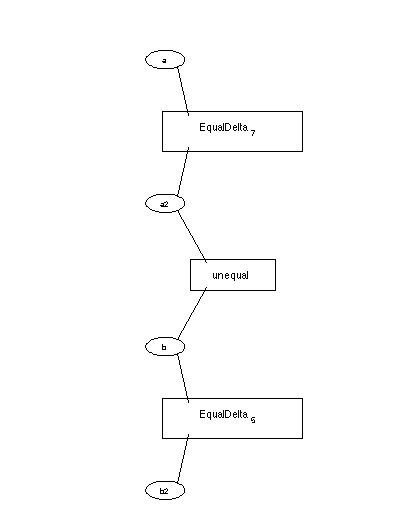
\includegraphics{images/SplitGraph.png}
 
Note that the split method takes a list of factors as the second through nth argument. This is the list of factors that will be moved from the original variable to the copied variable. All unspecified factors will remain connected to the initial variable.



\para{Joining Variables}

Users can now join variables. This will create a new joint variable and modify all factors connected to the original variables to reconnect to the new joint variable. This can be useful in eliminating loops in a graph. The following code creates a loopy graph and then uses join to remove the loop.

\begin{lstlisting}
a = Bit(); 
a.Name = 'a'; 
b = Bit();
b.Name  = 'b';
c = Bit();
c.Name = 'c';
d = Bit();
d.Name = 'd';

fg = FactorGraph();
f1 = fg.addFactor(@xorDelta,a,b,c);
f1.Name = 'xor';
f2 = fg.addFactor(@(x,y,z) (x|y)==z ,a,b,d);
f2.Name = 'or';
 
newvar = fg.join(a,b);
newvar.Name = 'a,b';

fg.plot(1);
\end{lstlisting}

The following is the loopy graph:

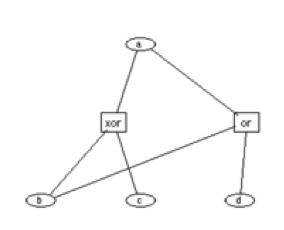
\includegraphics{images/LoopyGraph.png}
  
And after joining the variables we have:

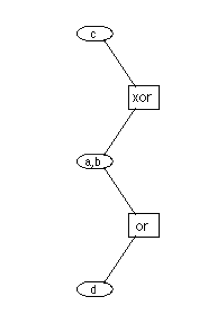
\includegraphics{images/NonLoopyGraph.png}

\para{Joining Factors}

Users can also join factors. It is possible to remove loops by joining factors as well as by joining variables.

\begin{lstlisting}
   b = Bit(4,1);
   for i = 1:4
       b(i).Name = sprintf('b%d',i);
   end
   fg = FactorGraph();
   f1 = fg.addFactor(@xorDelta,b(1:3));
   f2 = fg.addFactor(@xorDelta,b(2:4));
   
   f3 = fg.join(f1,f2);
   f3.Name = 'twoxors';
   
   b.Input = input;
   fg.solve();
   actualBelief = b.Belief;
   
   fg.plot(1);
\end{lstlisting}

The following plot shows the graph with the loops:  
 
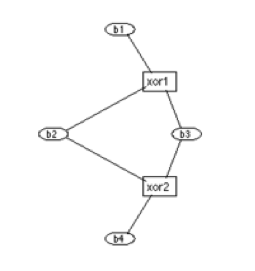
\includegraphics{images/LoopyGraph2.png}

And the following plot shows the graph after the factor is joined: 
 
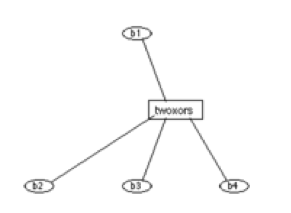
\includegraphics{images/NonLoopyGraph2.png}

To join factors, Dimple does the following:

\begin{itemize}
\item Find the variables in common between two factors.
\item Take the cartesian product of the tables but discard rows where the common variable indices differ.
\item Consolidate the columns with common variables.
\item Multiply the values for each row.
\end{itemize}



\subsubsection{Explicit Scheduling and Retrieving Message Values}

Dimple supports the ability to retrieve and set messages as well as to explicitly update edges, factors and variables.

\begin{lstlisting}
%OK, first we create a simple Factor Graph with a single xor connecting two  
%variables.
fg = FactorGraph(); 
b = Bit(2,1);
f = fg.addFactor(@xorDelta,b);
%We can go ahead and set some inputs
b(1).Input = .8;
b(2).Input = .7;


%we can examine some edges 
disp(f.Ports{1}.InputMsg);
disp(f.Ports{1}.OutputMsg);

%we can even set some edge messages
f.Ports{1}.InputMsg = [.6 .4];

%we can update a node 
b(1).update();
b(2).update();

%or all the variables in a vector.
b.update();

%or a specific edge
b(1).updateEdge(f);
 
%but updating via portNum is quicker
b(1).updateEdge(1);

%of course, if we don't know the portNum, we can get it
portNum = b(1).getPortNum(f);
b(1).updateEdge(portNum);

%We can do the same kind of stuff with factors
f.updateEdge(b(1));
f.updateEdge(f.getPortNum(b(2)));

%Let's look at some messages again
b(1).Ports{1}.InputMsg
b(2).Ports{1}.InputMsg

%and some beliefs
b.Belief
\end{lstlisting}



\subsubsection{Plotting}


When debugging Factor Graphs, it is sometimes useful to be able to plot a Factor Graph.  The FactorGraph class provides a plot method that can be used to visualize a Factor Graph.

The following code describes how to use the plot function in various ways.

\begin{lstlisting}
%First we build a Factor Graph to use for plotting examples
fg = FactorGraph();
b = Bit(6,1);
for i = 1:6
    b(i).Name = sprintf('b%d',i);
end
 
%We use Label rather than Name for the factors so that we can assign
%them the same Label.  Name must be a unique identifier,
%Label is just used for printing/plotting.
f1 = fg.addFactor(@xorDelta,b(1:4));
f1.Label = 'f';
f2 = fg.addFactor(@xorDelta,b(4:6));
f2.Label = 'f';
 
 
pause_time = 1;
 
%Calling plot with no arguments shows no labels.  It draws variables as
%circles and factors as squares.
fg.plot();
\end{lstlisting}

This will result in the following graph:


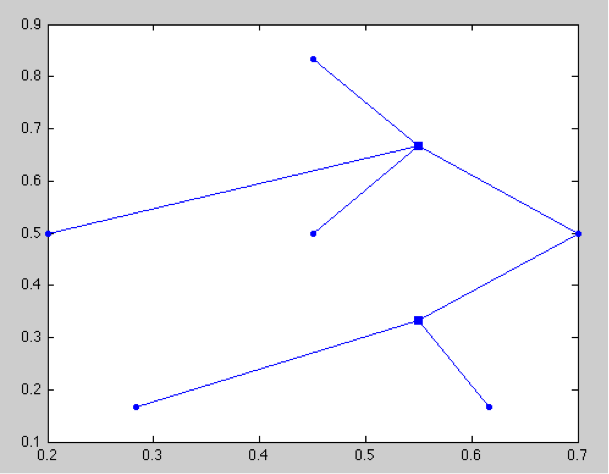
\includegraphics{images/plot1.png}

Note that factors are displayed as squares and variables as circles.

\begin{lstlisting}
pause(pause_time);
 
%The following is equivalent to the previous plot command.  We are simply
%explicitly turning off labels.
fg.plot('labels',false);
\end{lstlisting}

Results in the same plot as above.

\begin{lstlisting}
pause(pause_time);
 
%Now we turn on the labels.  Now we see the names we assigned to the
%various nodes and variables of the Factor Graph.
fg.plot('labels',true);
\end{lstlisting}

Results in the following:
 

 
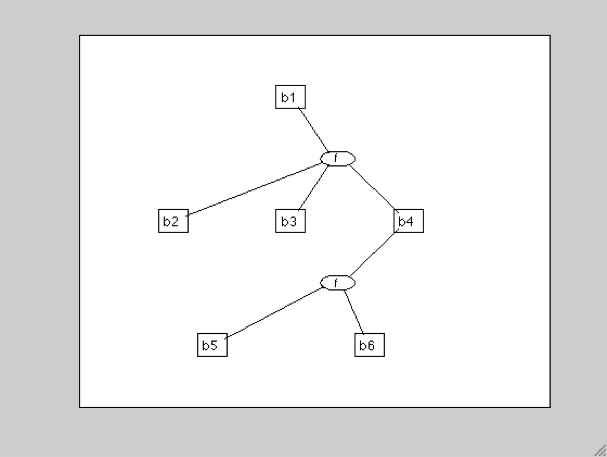
\includegraphics{images/plot2.png}

If the user has specified a Label, those will be displayed, otherwise the object�s Name�s will be displayed.


\begin{lstlisting}
pause(pause_time)
 
%We can specify a subset of nodes to plot
fg.plot('labels',1,'nodes',{b(1:2),f1});
\end{lstlisting}

Results in the following:



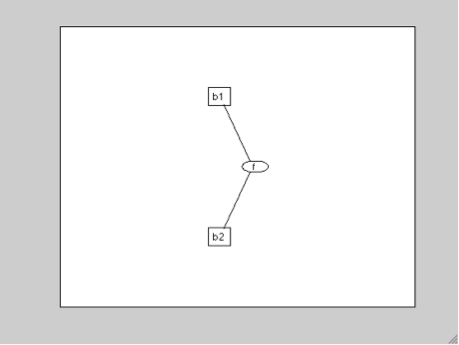
\includegraphics{images/plot3.png}

Only the specified nodes and their connectivity were included.

\begin{lstlisting}
pause(pause_time)
 
%By can set a global color for all the nodes in the graph.
fg.plot('labels',1,'color','g');
\end{lstlisting}

Setting a global color:



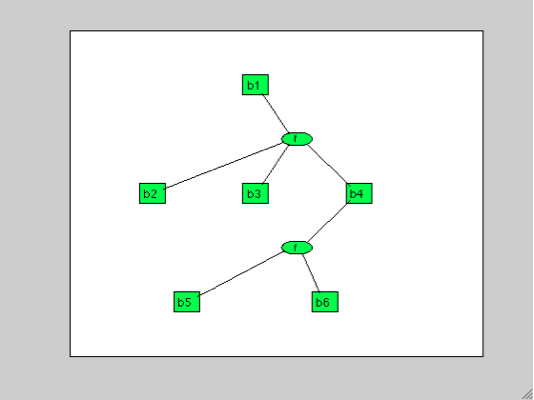
\includegraphics{images/plot4.png}

\begin{lstlisting}
pause(pause_time)
 
%We can specify a color for one node in the graph.
fg.plot('labels',1,'nodes',{b(1:2),f1},'color',b(1),'g');
\end{lstlisting}

Setting a color for a specific node:
 
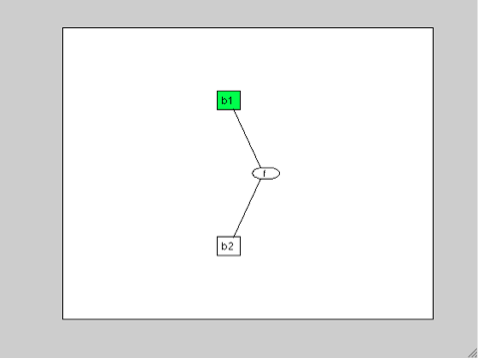
\includegraphics{images/plot5.png}
 
\begin{lstlisting}
pause(pause_time)
 
%We can specify colors for multiple nodes in the graph.
fg.plot('labels',1,'nodes',{b(1:2),f1},'color',{b(2),f1},{'r','c'});
\end{lstlisting}

Setting colors for multiple nodes:

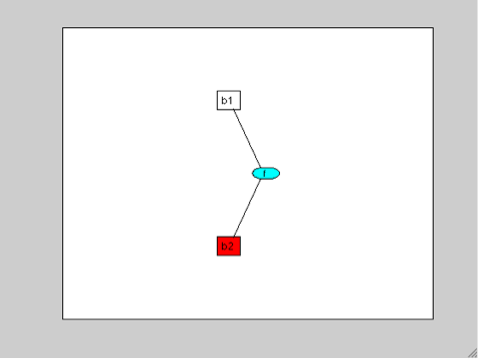
\includegraphics{images/plot6.png}

\begin{lstlisting}
pause(pause_time)
 
%We can mix setting a global color, colors for a single node mutliple
%times, and colors for multiple nodes.  The global color is used in all
%cases where a color has not explicitly been set for a node.
fg.plot('labels',1,'color',b(1),'g','color',b(2),'r','color',{b(3),b(4)},{'y','c'},'color','b');
\end{lstlisting}

Mixing and matching the various coloring options:

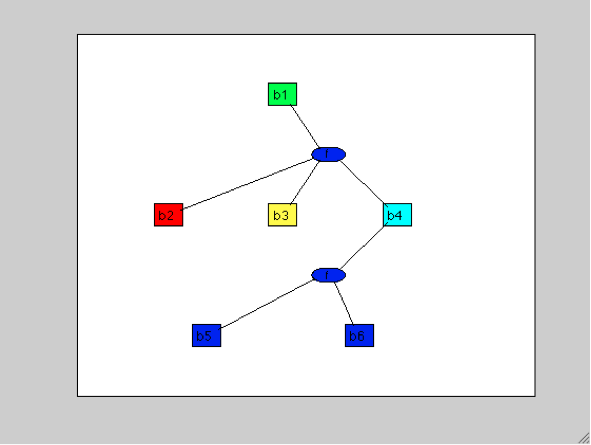
\includegraphics{images/plot7.png}

\begin{lstlisting}
pause(pause_time)
 
%We can also specify a root node on which we perform a depth first search
%up to a specific depth and then only print nodes up to that depth.
for depth = 0:5
 
    %Furthermore, we color the root node green so we know which is the root
    %node.
    fg.plot('labels',1,'depth',b(1),depth,'color',b(1),'g','color','b');
    
    pause(pause_time);
end
\end{lstlisting}

Specifying a depth will display a specified root node and all nodes that are N steps away.  The following shows the result of calling plot with �depth� of b(1) and 2:
 

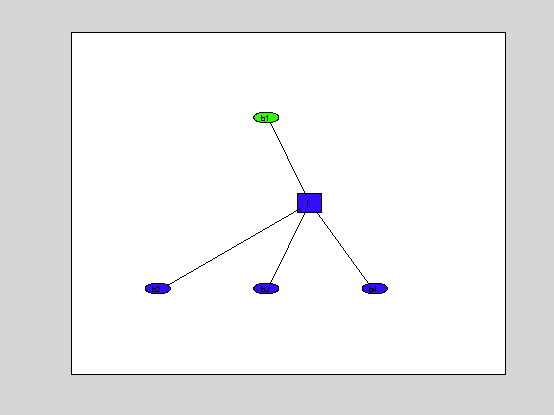
\includegraphics{images/plot8.png}

We also colored the root node green to make it clear which was the root node.

\begin{lstlisting}
%The following shows how using the depth feature we might be able to find
%out interesting information.  Here we increase the depth until we visually
%see a loop.
[ldpc,vars] = createLDPC();
v = vars(1);
 
for depth = 0:6
    ldpc.plot('depth',v,depth);
    
    pause(pause_time);
end
\end{lstlisting}

Here, we show how we can use plot to find interesting information about a large graph.  The final plot with a depth of 6 shows a cycle in an LDPC Factor Graph:

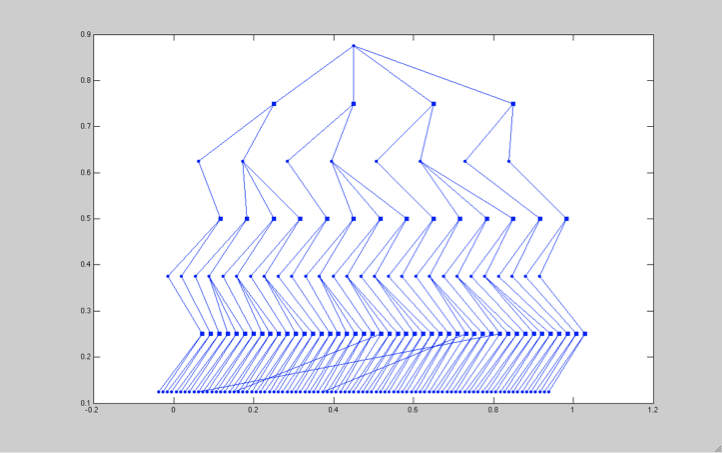
\includegraphics{images/plot9.png}

 
\para{Nesting}

By default, the plotting method ignores hierarchy and plots the flattened graph.  If the user specifies the 'nesting' parameter, however, they can specify how deep to descend into the hierarchy before considering NestedGraphs to be Factors and plotting them as such.

When labels are turned off, nested graphs are displayed as triangles

First let's build a graph with three levels of nesting.

\begin{lstlisting}
b = Bit(2,1);
template1 = FactorGraph(b);
iv = Bit();
template1.addFactor(@xorDelta,b(1),iv);
template1.addFactor(@xorDelta,b(2),iv);
 
b = Bit(2,1);
template2 = FactorGraph(b);
iv = Bit();
template2.addFactor(template1,b(1),iv);
template2.addFactor(template1,b(2),iv);
 
template2.plot();
 
b = Bit(2,1);
fg = FactorGraph(b);
iv = Bit();
fg.addFactor(template2,b(1),iv);
fg.addFactor(template2,b(2),iv);
\end{lstlisting}
 
Here we show the graph plotted with various levels of nesting.

fg.plot('nesting',0);

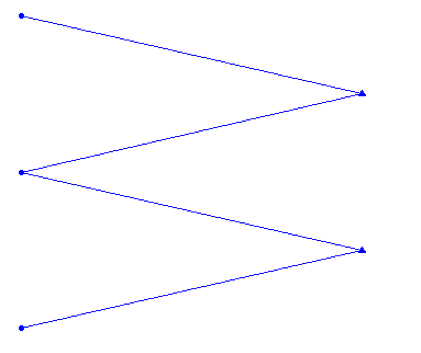
\includegraphics{images/plot10.png}


Notice the Nested Graphs show up as triangles.

\begin{lstlisting}
fg.plot('nesting',1);
\end{lstlisting}

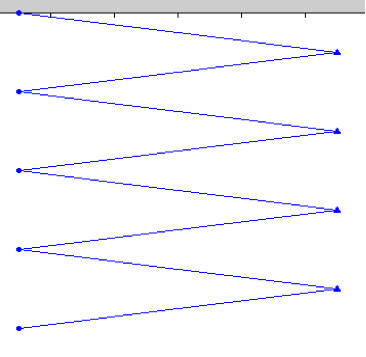
\includegraphics{images/plot11.png}
 
\begin{lstlisting}
fg.plot('nesting',2);
\end{lstlisting}


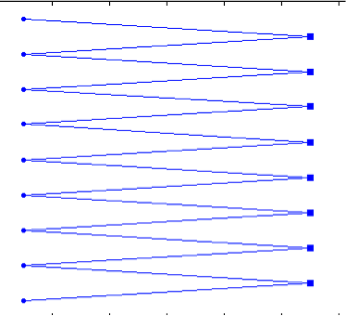
\includegraphics{images/plot12.png}
 
Note that once we�ve reached the bottom, we�re actually seeing the Factors plotted.
 
We can retrieve an instance of a nested graph and plot that with nesting set.

\begin{lstlisting}
fg.NestedGraphs{1}.plot('nesting',0);
pause(pause_time);
\end{lstlisting}



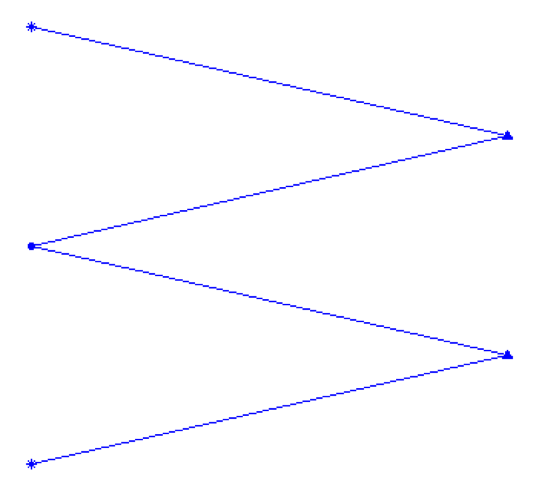
\includegraphics{images/plot13.png}
 
 
When plotting graphs, boundary variables show up as stars.

Next we mix depth first search with nesting


\begin{lstlisting}
fg.plot('nesting',0,'depth',iv,0);
\end{lstlisting}

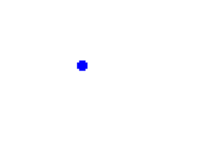
\includegraphics{images/plot14.png}
 

 
\begin{lstlisting}
fg.plot('nesting',0,'depth',iv,1);
\end{lstlisting}

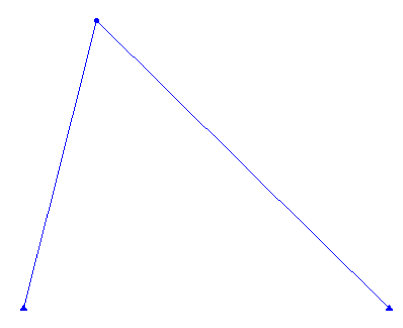
\includegraphics{images/plot15.png}
 

 
\begin{lstlisting}
fg.plot('nesting',0,'depth',iv,2);
\end{lstlisting}


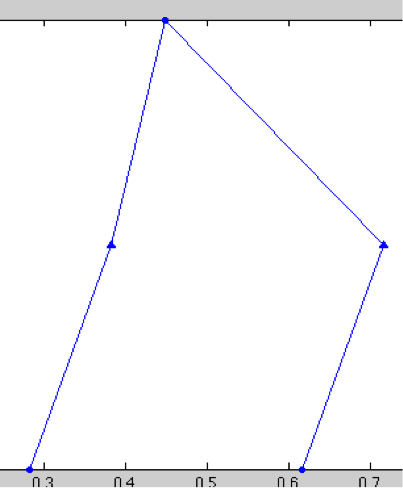
\includegraphics{images/plot16.png}




\subsubsection{Energy}

\para{Bethe Free Energy}

\[
BetheFreeEnergy = InternalEnergy - BetheEntropy
\]

\begin{lstlisting}
bfe = fg.BetheFreeEnergy;
\end{lstlisting}

\para{Internal Energy}

\[
 InternalEnergy = \sum_{a \in F }InternalEnergy(a) + \sum_{i \in V}InternalEnergy(i) 
 \]

Where F is the set of all Factors and V is the set of all variables.  If Dimple treated inputs as single node Factors, this method would only sum over factors.

\begin{lstlisting}
ie = fg.InternalEnergy;
\end{lstlisting}

\para{Bethe Entropy}

\[
 BetheEntropy = \sum_{a \in F}BetheEntropy(a) - \sum_{i \in V}BetheEntropy(i)(degree(i)-1) 
 \]

Where F is the set of all Factors and V is the set of all variables.

\begin{lstlisting}
be = fg.BetheEntropy;
\end{lstlisting}

\para{Factor Internal Energy}

\[
InternalEnergy(a) = \sum_{\vec{x} \in \vec{X}}B_a(\vec{x})*(-log(Weight(\vec{x}))) 
\]

Where a is an instance of a Factor, X is the set of variables connected to a, Weight is the FactorTable entry for the specified set of variable values, and B~a~ is the belief of that factor node.

\begin{lstlisting}
ie = f.InternalEnergy;
\end{lstlisting}

\para{Factor Bethe Entropy}

\[
BetheEntropy(a) = - \sum_{\vec{x} \in domain(\vec{X})}B_a(\vec{x})*log(B_a(\vec{x})) 
\]

Where a is an instance of a Factor, X is the set of variables connected to a, and B~a~ is the belief of that factor node.

\begin{lstlisting}
be = f.BetheEntropy;
\end{lstlisting}

\para{Variable Internal Energy}

\[
 InternalEnergy(i) = \sum_{d \in D}B_i(d)*(-log(Input(d))) 
 \]

Where D is variable i's domain and Input is the variable's input.

\begin{lstlisting}
ie = v.InternalEnergy;
\end{lstlisting}

\para{Variable Bethe Entropy}

\[
BentheEntropy(i) = - \sum_{d \in D}B_i(d)*log(B_i(d)) 
\]

Where D is variable i's domain.

\begin{lstlisting}
be = v.BetheEntropy();
\end{lstlisting}

Factor Belief

To support the Bethe Free Energy property, Dimple provides getBelief associated with a Factor.

\[
B_a(\vec{x}) = \frac{Weight(\vec{x})\prod_{i=0}^N \mu_{X_i \rightarrow a}(x_i)}{\sum_{\vec{x} \in \vec{X}}Weight(\vec{x})\prod_{i=0}^N \mu_{X_i \rightarrow a}(x_i\
)} 
\]

Where $ \vec{x} \in domain(\vec{X}) $ and $ \vec{X} $ is the set of variables connected to the factor a.

\begin{lstlisting}
b = f.Belief;
\end{lstlisting}

\para{Score}
\label{sec:score}

Users can retrieve the Energy of a Factor Graph, Variable Vector, or Factor. This feature is currently only supported with the SumProduct algorithm.

The following are examples of ways to retrieve the energy of FactorGraphs, factors, and variables:

\begin{lstlisting}
fg = FactorGraph();
b = Bit(3,1);
f = fg.addFactor(@xorDelta,b);

fg.Score
f.Score
b.Score
b(1).Score
\end{lstlisting}

When computing the score, the most likely variable value is used. It's possible to override that by setting a guess on a variable using:

\begin{lstlisting}
b.Guess = 1; %For other variable types, var.Guess takes a domain item.
\end{lstlisting}

\para{Math behind the score}

The variable energy is normalized by the maximum input probability.

\[
score(v) = -log(inputProb(guess) + log(max(inputProb)) 
\]

The factor energy is normalized by the largest factor value.

\[
score(f) = - log(f(guessxguessyguessz))+log(max(f)) 
\]

And the Factor Graph�s energy is as follows:

\[
score(fg) = \sum_{v \in V} score(v) + \sum_{f \in F} score(f) 
\]


\subsubsection{Introspection}

The FactorGraph class provides several feature for inspecting aspects of the graph.  The ability to nest graphs complicates things a bit.  Nested FactorGraphs can be considered Factors.  All of the introspection features allow the user to view nested graphs as leaf factors or to descend into them and operate on the children of the nested graphs.  Each feature provides several methods:

\begin{itemize}
\item $<$FeatureName$>$(int relativeNestingDepth) -- The relativeNestingDepth specifies how deep to descend into the nested FactorGraphs before treating deeper NestedGraphs as Factors.  Specifying 0 will treat the top level nested Graphs as factors.  Specifying a large enough number will descend all the way to the leaf factors.  Specifying something between 0 and the FactorGraph�s maximum depth will descend as far as this parameter specifies before considering NestedGraphs to be factors.  The parameter contains the word �relative� because users can retrieve nested graphs.  They can call one of the feature�s methods on that nested graph.  
\item $<$FeatureName$>$Flat() -- equivalent of $<$FeatureName$>$(max int)
\item $<$FeatureName$>$Top() -- equivalent of $<$FeatureName$>$(0)
\item $<$FeatureName$>$() -- equivalent of $<$FeatureName$>$Flat().  It was thought that users will most often want to operate on the FactorGraph in its flattened form.
\end{itemize}

Now, on to the specific features.

\para{Retrieving All Factors}

Users can retrieve Factors and/or NestedGraphs associated with a graph using the Factors methods and properties:

\begin{itemize}
\item Fg.Factors
\item Fg.FactorsFlat
\item Fg.FactorsTop
\item Fg.getFactors(relativeNestingDepth)
\end{itemize}

When the user specifies a relativeNestingDepth or calls FactorsTop, the resulting cell array will contain a mix of leaf factors and Nested Graphs.

\para{Retrieving Factors but not Nested Factor Graphs}

The FactorGraph class provides the following:

\begin{itemize}
\item NonFactorGraphFactors
\item NonFactorGraphFactorsFlat
\item NonFactorGraphFactorsTop
\item getNonFactorGraphFactors(relativeNestingDepth)
\end{itemize}

As the name implies, this will behave similar to the Factors properties and methods but will exclude nested graphs.

\para{Retrieving Variables}

The FactorGraph class provides the following:

\begin{itemize}
\item Variables -- calls VariablesFlat
\item VariablesFlat -- Returns a list of all the Variables in the graph, including those contained by nested graphs.
\item VariablesTop -- Returns only those variables contained in the top level of the graph.
\item getVariables(relativeNestingDepth,forceIncludeBoundaryVariables) -- Returns all variables contained in the FactorGraph from which the method is called as Variables that are as deep as the specified relativeNestingDepth.  The second parameter is optional and defaults to false.  When false, boundary variables are only included by the root graph.  When true, boundary variables are included regardless of whether a graph is a root or nested graph.
\end{itemize}

\para{Retrieving all Nodes}

The FactorGraph provides the following:

\begin{itemize}
\item Nodes
\item NodesFlat
\item NodesTop
\item getNodes(relativeNestingDepth,forceIncludeBoundaryVariables)
\end{itemize}

These methods call the Factor and Variable methods and concatenate the results together.

\para{Determining if a FactorGraph is a tree}

The FactorGraph class provides the following:

\begin{itemize}
\item isTree(relativeNestingDepth) 
\item isTreeTop 
\item isTreeFlat 
\end{itemize}


isTree -- Users can call <factor graph name>.isTree() to determine if a FactorGraph is a tree.  If the graph contains cycles, this method will return false. Like the other methods, the relativeNestingDepth determines at what point to consider NestedGraphs to be leaf cells.  

\para{Retrieving an Adjacency Matrix}

All of the following methods return a pair: [A, labels] where A is a square connectivity matrix and labels is a cell array of strings specifying the names of the nodes in A. 

\begin{itemize}
\item getAdjacencyMatrix(relativeNestingDepth,forceIncludeBoundaryVariables) -- relativeNestingDepth behaves the same as in other methods that take this parameter.  So does forceIncludeBoundaryVariables. forceIncludeBoundaryVariables has a default value of false.
\item getAdjacencyMatrix(nodes,forceIncludeBoundaryVariables) -- Users can specify a specific subset of nodes in which they�re interested.  This method will return an adjacency matrix with only those nodes.  Nodes are considered connected only if there is an edge directly connecting them.
\item getAdjacencyMatrixTop() -- equivalent to getAdjacencyMatrix(0,false)
\item getAdjacencyMatrixFlat() -- equivalent to getAdjacencyMatrix(intmax,false)
\end{itemize}

FactorGraph also provides an AdjacencyMatrix Property:

\begin{itemize}
\item AdjacencyMatrix -- equivalent to getAdjacencyMatrixFlat and only returns A (not the labels).  MATLAB properties can only return one object.
\end{itemize}

An example of getAdjacencyMatrix:

\begin{lstlisting}
fg = FactorGraph();
b = Bit(2,1);
b(1).Name = �b1�;
b(2).Name = �b2�;
f = fg.addFactor(@xorDelta,b);
f.Name = �f�;
[A,labels] = fg.getAdjacencyMatrix();
A =

     0     0     1
     0     0     1
     1     1     0


labels = 

    'b1'
    'b2'
    'f'
\end{lstlisting}

\para{Depth first search}

\begin{itemize}
\item depthFirstSearch(node, searchDepth, relativeNestingDepth) -- 
\begin{itemize}
\item node -- Specifies the node from which to initiate the search
\item searchDepth -- specifies how far from �node� the search should go.
\item relativeNestingDepth -- determines how deep to go down the NestedGraphs before considering NestedGraphs to be leaf cells. 
\end{itemize}
\item depthFirstSearchFlat(node, searchDepth) -- equivalent of depthFirstSearch(node,searchDepth,maxint)
\item depthFirstSearchThop(node, searchDepth) -- equivalent of depthFirstSearch(node,searchDepth,0)
\end{itemize}

An example:

\begin{lstlisting}
fg = FactorGraph();
b = Bit(6,1);
for i = 1:6
b(i).Name = sprintf('b%d',i);
end
f1 = fg.addFactor(@xorDelta,b(1:4));
f1.Name = 'f1';
f2 = fg.addFactor(@xorDelta,b(4:6));
f2.Name = 'f2';
 
nodes = fg.depthFirstSearch(b(1),3);
\end{lstlisting}

calling fg.plot(�color�,b(1),�g�,�labels�,true) reveals the following structure of this graph

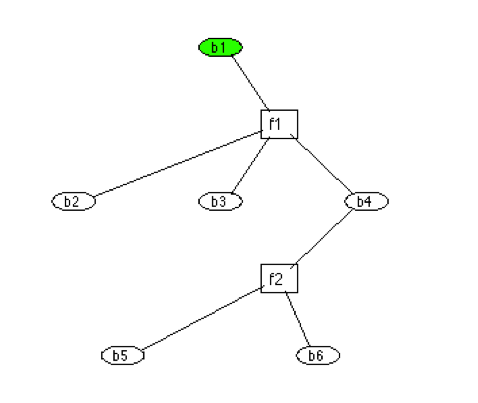
\includegraphics{images/Introspection.png}
 
As you might guess fg.depthFirstSearch(b(1),3) will return a collection of six nodes: b1, f1, b2, b3, b4, and f2.  It will not include b5 and b6 since those are at a depth of four from b1.

\subsubsection{Estimating Parameters}

Dimple provides support for estimating parameters.  Only the sumproduct solver currently supports this. 
The sum product algorithm computes the gradient of the BetheFreeEnergy and performs a gradient descent on this.  Users can
specify how many times to restart the gradient descent with random table values.

Users provide four arguments:

\begin{itemize}
\item factorsAndFactorTables - A cell array of FactorTables for which the user wants parameters to be estimated.  They can mix Factors and FactorTables
\item numRestarts - The number of times to randomly initialize the FactorTables and restart the gradient descent.
\item numSteps - The number of times to descend down along the gradient
\item stepScaleFactor - The value we scale the gradient by.
\end{itemize}

\begin{lstlisting}
fg.estimateParameters({factorTable1,factorTable2,factor1,etc...},numRestarts,numSteps,stepScaleFactor);
\end{lstlisting}

\subsubsection{Invoking Methods on the Underlying Solver Objects}

Users sometimes need access to the underlying solver objects in order to set and get
solver specific properties.  For instance K-best is implemented by minsum and sumproduct 
solvers.  

Let's use the following code to show examples of accessing underlying solver objects

\begin{lstlisting}
fg = FactorGraph();
d = Discrete(1:10,10,1);
ft = FactorTable(rand(10),d.Domain,d.Domain);
ft.normalize(1);
f = fg.addFactorVectorized(ft,d(1:(end-1)),d(2:end));
f.DirectedTo = d(2:end);
\end{lstlisting}

This code constructs a Markov Model of 10 variables with domain 1 through 10 and a randomized transition matrix.  Suppose we want to use K-best for all the factors.  We could access the underlying solver object of each factor and call setK on that object:

\begin{lstlisting}
for i = 1:length(f)
   f(i).Solver.setK(5);
end
\end{lstlisting}

However, in the case of very large graphs, this can be very inefficient.  MATLAB has a fairly large penalty for invoking function calls in a large for loop.  Instead, variables, factors, and factor graphs all have an invokeSolverMethod that can be used to call a method on all objects in the vector.

\begin{lstlisting}
f.invokeSolverMethod('setK',uint32(5));
\end{lstlisting}

After this is invoked, all factors will have K set to 5.  There are two issues with the current implementation that should be fixed at some point.  The first is that it currently only supports providing the same values to all solver objects.  If you wanted to set a different K for all factors, you could not use this mechanism.  The second issue is that, users must be careful to correctly cast their arguments to the appropriate types.  This could and should be fixed.

It's also possible to call methods with return values as follows:

\begin{lstlisting}
d.invokeSolverMethod('setDamping',uint32(0),2.0);
damping = d.invokeSolverMethodWithReturnValue('getDamping',uint32(0));

damping

>> damping

damping = 

    [2]
    [2]
    [2]
    [2]
    [2]
    [2]
    [2]
    [2]
    [2]
    [2]

\end{lstlisting}

Here we set the damping value for the first edge of every variable.




